\section{Online Rewrite Engine}
\label{sec:query_rewriting}
The Rewrite Engine rewrites each incoming query with the rule set $\mathcal{R}$, the Fragment Index $\mathit{FI}$, and the rule ordering $\omega$, without calls to LLMs.
We describe its rule selection and application, and unparsing, as well as rewriting of new queries and remaining limitations.

\vspace{-0.25cm}
\subsection{Rule Selection}
\label{sec:online:fragment}
Checking every rule in $\mathcal{R}$ on every node of the plan $P(Q)$ costs $O(|\mathcal{R}| \cdot |P(Q)|)$ evaluations of $\phi_r$ per query, which would scale with the rule set. Our Fragment Index avoids this linear scaling. The engine traverses $P(Q)$ once and computes the fragment keys of the subtrees rooted at each node, up to a maximum depth $d$. It uses the same key extractor that registers rules in $\mathit{FI}$, so equal fragments yield equal keys. We only evaluate applicable rules $\phi_r$ via hash lookups in $\mathit{FI}$ per key. Thus, selection costs $O(d \cdot |P(Q)|)$ lookups, and application cost grows with $|\mathcal{R}(Q)|$, not with $|\mathcal{R}|$. If $\mathcal{R}(Q)$ is empty, the query passes through unaltered.

\vspace{-0.25cm}
\subsection{Rule Application and Ordering}
\label{sec:online:apply}
The rule order can affect the rewriting. A rule that fires early can change the plan into a shape that blocks a more useful rule later. {\sys} therefore applies $\mathcal{R}(Q)$ in the ordering $\omega$, by default the descending priority order of the rules (Line~\ref{pipeline:order} of Algorithm~\ref{alg:pipeline}). This priority order was assigned by the LLM during distillation (Section~\ref{sec:offline:distill}) and is deterministic without a need for search.

\begin{algorithm}[t]\fontsize{7.9}{9.5}\selectfont
\caption{\textsf{ApplyRules}$(P,\, \mathcal{R}(Q),\, \omega)$}
\label{alg:apply}
\begin{algorithmic}[1]
\REQUIRE logical plan $P$, applicable rules $\mathcal{R}(Q)$, rule ordering $\omega$
\ENSURE rewritten plan $P$
\STATE \label{apply:sort} $\mathcal{R}_\omega \leftarrow \textsf{Sort}(\mathcal{R}(Q),\, \omega)$
\STATE $\mathit{changed} \leftarrow \mathbf{true}$;\quad $\mathit{iter} \leftarrow 0$
\WHILE{\label{apply:while} $\mathit{changed}$ \AND $\mathit{iter} < \textsc{MaxIter}$}
  \STATE $\mathit{changed} \leftarrow \mathbf{false}$
  \FOR[bottom-up, top-down]{\label{apply:pass} $\textsf{Visit} \in \langle \textsf{PostOrder}, \textsf{PreOrder} \rangle$}
    \FOR{node $v \in \textsf{Visit}(P)$}
      \FOR{$r \in \mathcal{R}_\omega$}
        \IF{$r.\textsf{Matches}(v)$}
          \STATE \label{apply:fire} $v \leftarrow r.\textsf{Apply}(v)$
          \STATE $\mathit{changed} \leftarrow \mathbf{true}$;\quad \textbf{break} \algorithmiccomment{first match only}
        \ENDIF
      \ENDFOR
    \ENDFOR
  \ENDFOR
  \STATE $\mathit{iter} \leftarrow \mathit{iter} + 1$
\ENDWHILE
\RETURN $P$
\end{algorithmic}
\end{algorithm}


\begin{figure*}[!t]
\vspace{-0.25cm}
    \centering
    \resizebox{.99\textwidth}{!}{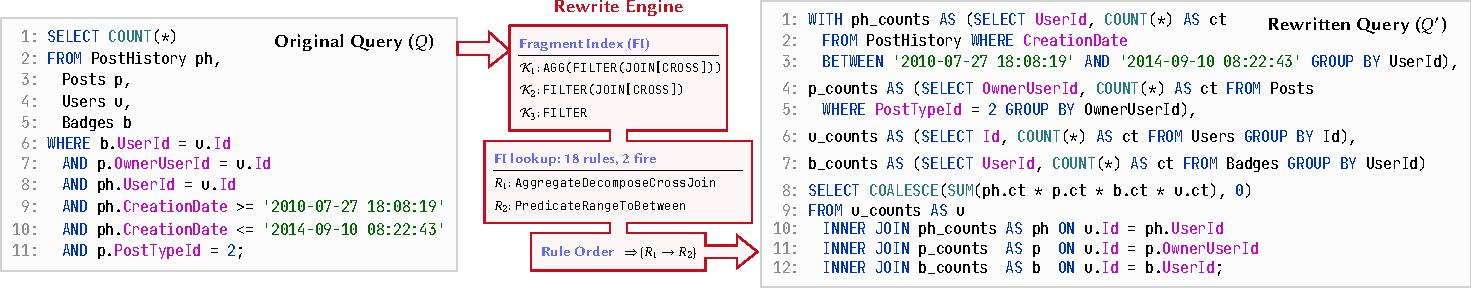
\includegraphics[scale=1]{figures/img/fig_StatsQ122Rewrite}}
    \vspace{-0.35cm}
    \caption{Online rewriting of Stats-CEB query~122: \blue{the Fragment Index retrieves 18 Stats-CEB rules through shared fragment keys; in priority order $\omega$, \texttt{AggregateDecomposeCrossJoin} and \texttt{PredicateRangeToBetween} fire and yield $Q'$.}}
    \label{fig:rewrite:example}
    \vspace{-0.35cm}
\end{figure*}


\textbf{Optional MCTS Search:}
\label{sec:online:mcts}
{\sys} can further optionally search for an optimal rule order per query with Monte Carlo Tree Search (MCTS)~\cite{learnedrewrite}.
Nodes of the search tree are rewritten plans, edges are rule applications, and we select nodes by the UCB1 criterion~\cite{Auer02}:
\begin{equation}
\mathrm{UCB1}(v) = \frac{G(v)}{T(v)} + c \cdot \sqrt{\frac{\ln T(\mathrm{parent}(v))}{T(v)}},
\end{equation}
where $G(v)$ is the cumulative reward of node $v$, $T(v)$ its visit count, and $c > 0$ the exploration constant.
The reward of a node is $\max\bigl(0, (C_{\mathrm{root}} - C_{v})/C_{\mathrm{root}}\bigr)$, where $C$ is the estimated plan cost.
The engine first rewrites the query in priority order; the searched plan must then reduce estimated cost by at least $5\%$ and pass a SQL validity check. If the priority pass has fired rules whose benefit cannot be estimated (e.g., a semijoin lift that avoids join blow-up), the engine keeps the priority plan and skips searching. With a budget of 100 iterations, the search takes only tens of milliseconds per query.
% TODO(Saeed, Q3): does MCTS run online per query or offline once? If online, drop "on the sampled queries Q_s" and "computes offline" above, and say MCTS searches each query's plan at rewrite time. If offline, state in one sentence how the per-query sequences become the single ordering omega.
% Sec. 6: replace "the anti-regression guard of Section ??" with "the adoption rule of Section~\ref{sec:online:apply}", and apply it to SOLEX-MCTS only.

\textbf{Cost Estimation:}
\label{sec:online:cost}
The estimated cost of a plan is the sum of the output cardinalities of its operators ($C_{out}$).
{\sys} estimates these cardinalities without running any query.
It propagates the number of distinct values (NDV) of each column bottom-up through the plan.
Join selectivity is $1/\max(\mathrm{NDV}(A.k), \mathrm{NDV}(B.k))$~\cite{Selinger79}.
Filter selectivity is $1/\mathrm{NDV}(\texttt{col})$ for a point predicate and $\min(0.5, n/\mathrm{NDV}(\texttt{col}))$ for an \texttt{IN}-list of $n$ values~\cite{Lohman88}.
After each join and filter, {\sys} updates the NDV of every output column~\cite{NeumannM11}.
An aggregate outputs $\min(|\mathit{child}|, \prod_i \mathrm{NDV}(\texttt{group}_i))$ rows.
This estimate may not align with the host optimizer, so priority order is the default.

\textbf{Fixed-Point Application:}
Algorithm~\ref{alg:apply} applies the ordered rules to the plan $P$ of a query.
Line~\ref{apply:sort} sorts $\mathcal{R}(Q)$ by $\omega$ once per query.
The outer loop (Line~\ref{apply:while}) repeats until no rule fires anymore or the budget \textsc{MaxIter} is reached, which guarantees termination if there are cyclic rule applications.
Each iteration runs two passes over the plan (Line~\ref{apply:pass}).
At each node, the first rule in $\mathcal{R}_\omega$ whose \texttt{Matches()} fires, and the pass moves to the next node (Line~\ref{apply:fire}). So only the first rule fires on a node.
The \emph{bottom-up pass} visits children before their parent. It suits \emph{push-down} rules, such as predicate and projection push-down, which move operators toward the scans. Each child is rewritten before its parents.
In reverse, the \emph{top-down pass} visits a parent before its children. It suits \emph{pull-up} rules, such as aggregation hoisting and join factorization. These rules must see the surrounding plan before they restructure the subtrees below.
Finally, the engine unparses the rewritten plan into the target SQL dialect.


\subsection{Rewriting Unseen Queries}
\label{sec:online:e2e}
Rules distilled from a query fire on queries with other characteristics.
Figure~\ref{fig:rewrite:example} and Example~\ref{example:online_rewrite} trace query~122 with the Stats-CEB rules.

% TODO(Saeed, Q5, blocking): Fig. 5 drops Users from Q', but JoinDecomposeToPreaggregatedCount keeps the anchor (Figs. 11-12).
% Send the engine's actual output for query 122, and check line 7 of Q against the Stats schema (PostHistory vs. Posts.OwnerUserId).
% Then revise the JoinReorder sentence below ("moves the scan of Users first") to match the output.
\vspace{-0.25cm}
\begin{example}[Online Rewriting]
\label{example:online_rewrite}
\sloppy
Query~122 joins \texttt{Post\allowbreak History}, \texttt{Posts}, and \texttt{Badges} with the anchor table \texttt{Users}.
It shares only \texttt{Badges} and \texttt{Users} with query~88.
Its plan contains the fragment keys \texttt{AGG(\allowbreak FILTER(\allowbreak JOIN[CROSS]))} and \texttt{FILTER(\allowbreak JOIN[CROSS])}, so the Fragment Index returns 18 Stats-CEB rules, and the engine tries them in priority order. Two of them fire: \texttt{AggregateDecompose\allowbreak CrossJoin} (priority 80) performs the same factorization as \texttt{JoinDecomposeTo\allowbreak Preaggregated\allowbreak Count} in Example~\ref{ex:1} and fires first because of its priority. Once the join is rewritten, the patterns of the lower-priority join rules, such as \texttt{FilterIntoJoin} and \texttt{JoinReorder}, no longer match, and only \texttt{PredicateRange\allowbreak ToBetween} (priority 10) still fires.
Query~122 differs from query~88 in three ways.
\emph{(i) Arity:}
Query~88 has two branches, and query~122 has three.
No rule fixes the number of branches.
\texttt{AggregateDecompose\allowbreak CrossJoin} builds one CTE per branch, \texttt{ph\_\allowbreak counts}, \texttt{p\_\allowbreak counts}, and \texttt{b\_\allowbreak counts}, plus \texttt{u\_\allowbreak counts} for the anchor.
It rewrites the root to \texttt{SUM(ph.ct\,$\times$\allowbreak\,p.ct\,$\times$\allowbreak\,b.ct\,$\times$\allowbreak\,u.ct)} over joins that start from \texttt{u\_\allowbreak counts}.
\emph{(ii) Tables:}
The rules have never seen \texttt{Post\allowbreak History} and \texttt{Posts}, do not encode their names, and thus, build the CTEs for matching branches.
\emph{(iii) Predicates:}
Query~122 filters \texttt{Post\allowbreak History} and \texttt{Posts}, and none of these filters appears in query~88.
\texttt{AggregateDecompose\allowbreak CrossJoin} then pushes the filters of each branch into the CTE of that branch independent of column names or constants, and \texttt{PredicateRange\allowbreak ToBetween} then turns the two bounds on \texttt{CreationDate} into a \texttt{BETWEEN}.
\end{example}

\vspace{-0.35cm}
\subsection{Limitations and Future Work}
\label{sec:limitations}

{\sys} has four remaining limitations which are future work.

\textbf{(1) Formal Coverage:}
Rules whose query pairs the solver cannot decide are admitted by result-equivalence tests on samples.
Proving the rule pattern itself, rather than query pairs, would let one proof cover every query a rule matches, including on new schemas.

\textbf{(2) Discovery Latency:}
A query with new patterns runs unchanged until the next offline batch distillation.
Running the generator continuously on monitored queries would reduce latency.

\textbf{(3) Cost-aware Ordering:}
The priority order ignores the host's cost model.
Ordering rules and discarding redundant rules, with feedback from the host optimizer, is a promising direction.

\textbf{(4) Beyond the Logical Layer:}
{\sys} rewrites only the logical plans and leaves physical design tuning to the host.
Distilling reusable physical hints, such as index or join-method choices, from the same LLM discoveries is a natural extension.
